\section{Methodology}
\label{sec:methodology}

This section presents the RTXGNN (Real-Time Explainable Graph Neural Network) framework, a novel architecture that jointly optimizes fraud detection accuracy and explanation quality through intrinsic interpretability mechanisms. We first formalize the problem (Section~\ref{subsec:problem}), then detail our two core innovations: Hierarchical Recency-Aware Positional Encoding (HRAPE, Section~\ref{subsec:hrape}) and Self-Explainable Aggregation Layer (SEAL, Section~\ref{subsec:seal}). Finally, we describe the training procedure with multi-task learning objectives (Section~\ref{subsec:training}). The architecture of RTXGNN is presented in Figure \ref{fig:architecture}. In this figure, the framework processes temporal transaction graphs through three main stages: (1) Hierarchical Recency-Aware Positional Encoding (HRAPE) captures multi-scale temporal patterns through recency decay, periodicity, and velocity features; (2) Self-Explainable Aggregation Layers (SEAL) generate sparse differentiable masks for features, edges, and nodes while performing message passing across L=3 layers; (3) Dual-head output produces both fraud predictions (ŷ) and multi-granularity explanations (M\textsuperscript{feat}, M\textsuperscript{edge}, M\textsuperscript{node}, M\textsuperscript{temp}) simultaneously without post-hoc optimization.

\begin{figure}[h]
\centering
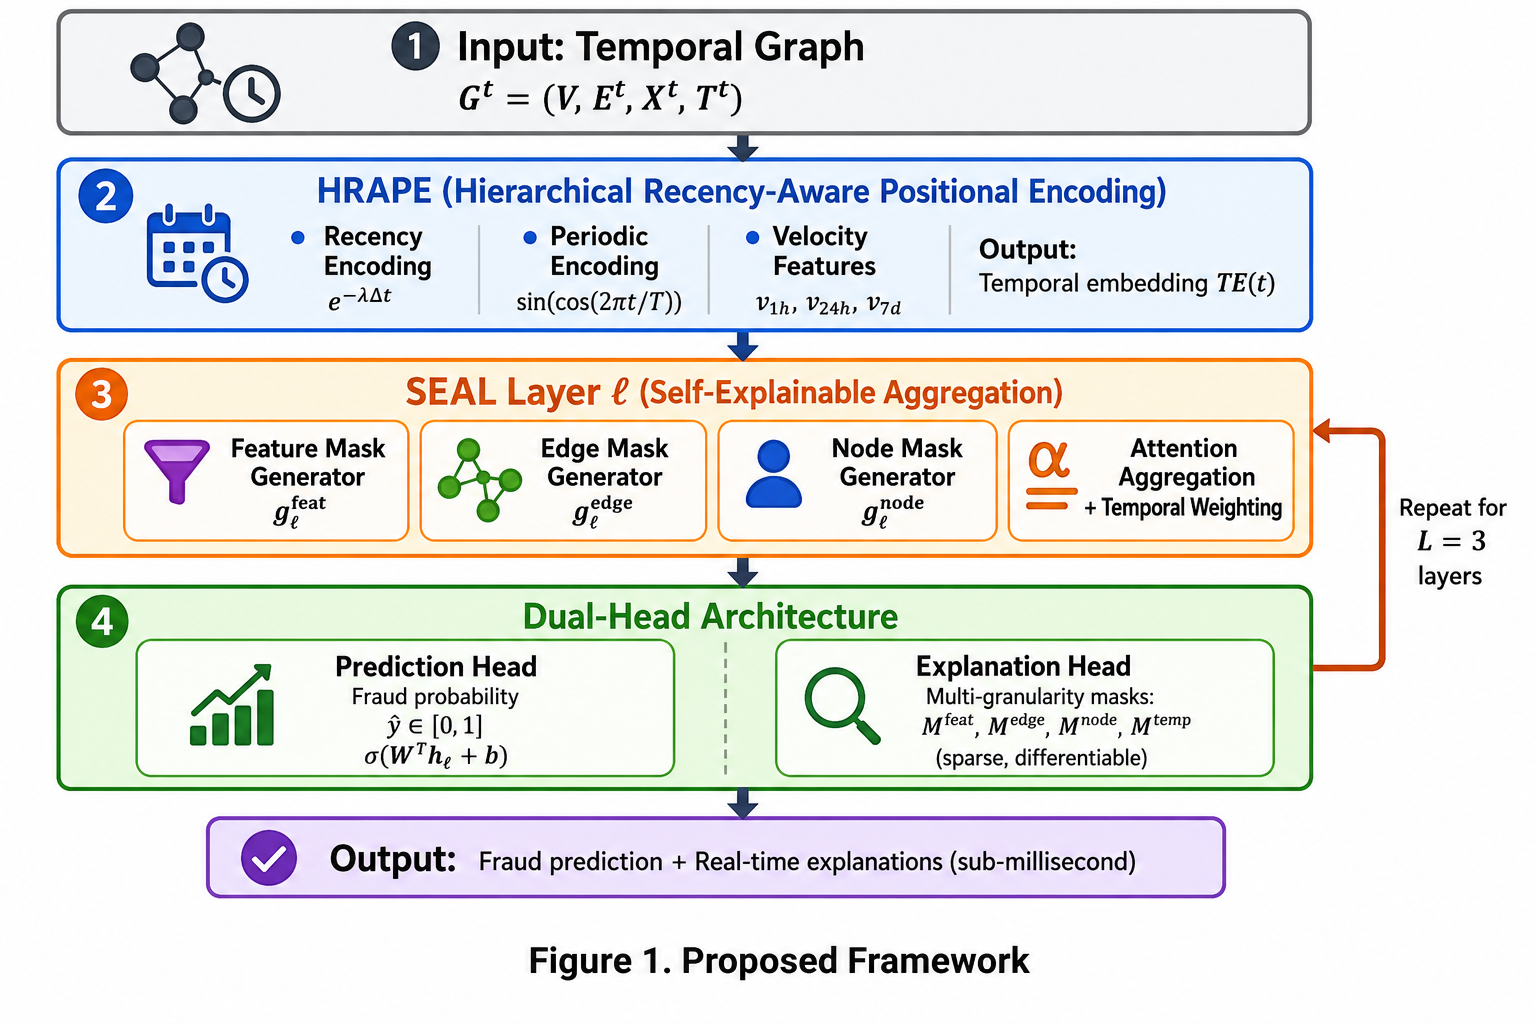
\includegraphics[width=\columnwidth]{rtxgnn_diagram.png}
\caption{RTXGNN architecture overview.}
\label{fig:architecture}
\end{figure}

\subsection{Problem Formulation}
\label{subsec:problem}

We model the financial transaction network as a dynamic temporal graph $\mathcal{G}^t = (\mathcal{V}, \mathcal{E}^t, \mathbf{X}^t, \mathbf{T}^t)$ at time $t$, where:

\begin{itemize}
    \item $\mathcal{V} = \{v_1, \ldots, v_n\}$ is the set of $n$ entities (accounts, addresses, wallets);
    \item $\mathcal{E}^t \subseteq \mathcal{V} \times \mathcal{V}$ is the set of directed edges representing transactions at time $t$;
    \item $\mathbf{X}^t \in \mathbb{R}^{n \times d_v}$ is the node feature matrix, where each row $\mathbf{x}_i \in \mathbb{R}^{d_v}$ contains behavioral and structural features for node $v_i$;
    \item $\mathbf{T}^t \in \mathbb{R}^{|\mathcal{E}^t|}$ contains timestamps for each edge in $\mathcal{E}^t$.
\end{itemize}

\noindent\textbf{Fraud Detection Task:} Given a target node $v_i$ (representing a transaction or account), predict the probability that $v_i$ is involved in fraudulent activity:
\begin{equation}
    \hat{y}_i = f_\theta(\mathcal{G}^t, v_i) \in [0, 1]
\end{equation}
where $\theta$ denotes the model parameters.

\noindent\textbf{Explanation Generation Task:} Simultaneously generate a multi-granularity explanation $\mathcal{X}_i = \{\mathbf{M}^{\text{node}}_i, \mathbf{M}^{\text{edge}}_i, \mathbf{M}^{\text{feat}}_i, \mathbf{M}^{\text{temp}}_i\}$ comprising:

\begin{itemize}
    \item $\mathbf{M}^{\text{node}} \in [0,1]^n$: Node importance scores indicating which neighbors contribute to the prediction;
    \item $\mathbf{M}^{\text{edge}} \in [0,1]^{|\mathcal{E}^t|}$: Edge importance scores identifying critical transaction paths;
    \item $\mathbf{M}^{\text{feat}} \in [0,1]^{d_v}$: Feature importance scores revealing which attributes drive the decision;
    \item $\mathbf{M}^{\text{temp}} \in [0,1]^{|\mathcal{E}^t|}$: Temporal importance scores capturing timing-dependent patterns.
\end{itemize}

The joint optimization objective is:
\begin{equation}
    \min_\theta \mathcal{L}_{\text{pred}}(\hat{y}, y) + \lambda_{\text{exp}} \mathcal{L}_{\text{exp}}(\mathcal{X}) + \lambda_{\text{sparse}} \mathcal{L}_{\text{sparse}}(\mathcal{X})
\end{equation}
where $\mathcal{L}_{\text{pred}}$ measures prediction accuracy, $\mathcal{L}_{\text{exp}}$ ensures explanation fidelity, and $\mathcal{L}_{\text{sparse}}$ promotes concise explanations through sparsity regularization. Hyperparameters $\lambda_{\text{exp}}$ and $\lambda_{\text{sparse}}$ balance the three objectives.

\subsection{Hierarchical Recency-Aware Positional Encoding (HRAPE)}
\label{subsec:hrape}

Temporal patterns are critical in fraud detection—fraudsters exploit velocity attacks (rapid transaction sequences), dormancy reactivation (sudden activity after inactivity), and coordinated timing. Unlike existing temporal GNNs that use simple timestamp concatenation or single-scale encodings, HRAPE captures multi-scale temporal dynamics through a hierarchical encoding scheme combining recency weighting and periodic patterns.

\subsubsection{Multi-Scale Temporal Features}

For each edge $e_{ij} = (v_i, v_j, t_{ij})$ with timestamp $t_{ij}$, we compute temporal features at multiple scales:

\paragraph{Recency Encoding:} We model temporal decay using an exponential function with learnable decay rate $\lambda \in \mathbb{R}^+$:
\begin{equation}
    r(t_{ij}, t) = \exp\left(-\lambda (t - t_{ij})\right)
\end{equation}
where $t$ is the current time step. This ensures recent transactions receive higher weights, critical for detecting burst patterns.

\paragraph{Periodic Encoding:} Financial fraud exhibits cyclical patterns (e.g., end-of-month salary transfers, weekend dormancy). We capture periodicity at multiple granularities using sinusoidal functions:
\begin{align}
    \mathbf{p}_{\text{hour}}(t) &= \left[\sin\left(\frac{2\pi \cdot h(t)}{24}\right), \cos\left(\frac{2\pi \cdot h(t)}{24}\right)\right] \\
    \mathbf{p}_{\text{day}}(t) &= \left[\sin\left(\frac{2\pi \cdot d(t)}{7}\right), \cos\left(\frac{2\pi \cdot d(t)}{7}\right)\right] \\
    \mathbf{p}_{\text{month}}(t) &= \left[\sin\left(\frac{2\pi \cdot m(t)}{30}\right), \cos\left(\frac{2\pi \cdot m(t)}{30}\right)\right]
\end{align}
where $h(t)$, $d(t)$, and $m(t)$ extract hour-of-day, day-of-week, and day-of-month from timestamp $t$.

\paragraph{Velocity Features:} We compute transaction velocities at multiple time windows to detect burst patterns:
\begin{align}
    v_{1h}(v_i, v_j) &= \frac{\text{count}\{e \in \mathcal{E} : \text{src}(e) = v_i, \text{tgt}(e) = v_j, t - t_e \leq 1h\}}{1} \\
    v_{24h}(v_i, v_j) &= \frac{\text{count}\{e \in \mathcal{E} : \text{src}(e) = v_i, \text{tgt}(e) = v_j, t - t_e \leq 24h\}}{24} \\
    v_{7d}(v_i, v_j) &= \frac{\text{count}\{e \in \mathcal{E} : \text{src}(e) = v_i, \text{tgt}(e) = v_j, t - t_e \leq 7d\}}{168}
\end{align}

We also compute acceleration (velocity change rate) to detect sudden shifts:
\begin{equation}
    a(v_i, v_j) = \frac{v_{1h}(v_i, v_j) - v_{24h}(v_i, v_j)}{v_{24h}(v_i, v_j) + \epsilon}
\end{equation}
where $\epsilon = 10^{-6}$ prevents division by zero.

\subsubsection{Learnable Hierarchical Encoding}

We combine raw temporal features through learnable transformations at each scale $s \in \{\text{hour}, \text{day}, \text{week}, \text{month}\}$:
\begin{equation}
    \mathbf{TE}_s(t) = \mathbf{W}_s \boldsymbol{\phi}_s(t) + \mathbf{b}_s
\end{equation}
where $\boldsymbol{\phi}_s(t)$ denotes the Fourier features at scale $s$, and $\mathbf{W}_s \in \mathbb{R}^{d_{\text{te}} \times d_\phi}$, $\mathbf{b}_s \in \mathbb{R}^{d_{\text{te}}}$ are learnable parameters. The final temporal encoding aggregates across scales:
\begin{equation}
    \mathbf{TE}(t) = \sum_{s \in \{\text{hour}, \text{day}, \text{week}, \text{month}\}} \mathbf{TE}_s(t)
\end{equation}

This hierarchical design allows the model to learn which temporal scales are most relevant for fraud detection, adapting to dataset-specific patterns.

\subsubsection{Recency-Weighted Attention}

HRAPE influences message-passing through recency-weighted attention. For an edge $(v_i, v_j)$ with timestamp $t_{ij}$, the attention coefficient is computed as:
\begin{equation}
    \alpha_{ij} = \frac{\exp\left(\frac{(\mathbf{W}_Q \mathbf{h}_i)^\top (\mathbf{W}_K \mathbf{h}_j)}{\sqrt{d_k}} + \gamma \cdot r(t_{ij}, t)\right)}{\sum_{v_k \in \mathcal{N}(v_i)} \exp\left(\frac{(\mathbf{W}_Q \mathbf{h}_i)^\top (\mathbf{W}_K \mathbf{h}_k)}{\sqrt{d_k}} + \gamma \cdot r(t_{ik}, t)\right)}
\end{equation}
where $\mathbf{W}_Q, \mathbf{W}_K \in \mathbb{R}^{d_k \times d}$ are query and key projection matrices, $\mathbf{h}_i, \mathbf{h}_j$ are node embeddings, and $\gamma \in \mathbb{R}^+$ is a learnable temperature parameter controlling the influence of recency. This formulation ensures that recent transactions receive higher attention weights during aggregation, enabling the model to prioritize temporally relevant information.

\subsection{Self-Explainable Aggregation Layer (SEAL)}
\label{subsec:seal}

The core innovation of RTXGNN is the Self-Explainable Aggregation Layer (SEAL), which generates explanations intrinsically during message-passing rather than requiring post-hoc optimization. SEAL jointly learns node representations and differentiable importance masks through three parallel mask generators operating at different granularities.

\subsubsection{Architecture Overview}

Each SEAL layer $\ell \in \{1, \ldots, L\}$ maintains three types of learnable mask generators:

\begin{itemize}
    \item \textbf{Feature Mask Generator} $g^{\text{feat}}_\ell: \mathbb{R}^{d_\ell} \to [0,1]^{d_\ell}$ identifies which input features are important;
    \item \textbf{Edge Mask Generator} $g^{\text{edge}}_\ell: \mathbb{R}^{2d_\ell} \to [0,1]$ determines which edges contribute to predictions;
    \item \textbf{Node Mask Generator} $g^{\text{node}}_\ell: \mathbb{R}^{d_\ell} \to [0,1]$ scores the importance of each node in the computation graph.
\end{itemize}

Each generator is implemented as a two-layer MLP with sigmoid activation:
\begin{equation}
    g(\mathbf{x}) = \sigma(\mathbf{W}_2 \cdot \text{ReLU}(\mathbf{W}_1 \mathbf{x} + \mathbf{b}_1) + \mathbf{b}_2)
\end{equation}
where $\sigma$ is the sigmoid function ensuring outputs lie in $[0,1]$.

\subsubsection{Forward Pass with Mask Generation}

The forward pass of SEAL layer $\ell$ proceeds as follows:

\paragraph{Step 1 - Feature Masking:} Given input embeddings $\mathbf{H}^{(\ell-1)} \in \mathbb{R}^{n \times d_{\ell-1}}$, generate feature masks:
\begin{equation}
    \mathbf{M}^{\text{feat},(\ell)} = g^{\text{feat}}_\ell(\mathbf{H}^{(\ell-1)})
\end{equation}

Apply masks element-wise to identify important features:
\begin{equation}
    \tilde{\mathbf{H}}^{(\ell-1)} = \mathbf{H}^{(\ell-1)} \odot \mathbf{M}^{\text{feat},(\ell)}
\end{equation}
where $\odot$ denotes element-wise multiplication.

\paragraph{Step 2 - Message Computation with Edge Masking:} For each edge $(v_i, v_j) \in \mathcal{E}$, compute edge representation:
\begin{equation}
    \mathbf{e}_{ij} = \left[\tilde{\mathbf{h}}^{(\ell-1)}_i \| \tilde{\mathbf{h}}^{(\ell-1)}_j\right]
\end{equation}
where $\|$ denotes concatenation.

Generate edge mask and temporal weight:
\begin{align}
    m_{ij}^{\text{edge}} &= g^{\text{edge}}_\ell(\mathbf{e}_{ij}) \\
    w_{ij}^{\text{temp}} &= \text{TemporalScorer}(\mathbf{TE}(t_{ij}))
\end{align}

The temporal scorer is a learned function mapping temporal encodings to importance weights:
\begin{equation}
    \text{TemporalScorer}(\mathbf{TE}) = \sigma(\mathbf{w}_{\text{temp}}^\top \mathbf{TE} + b_{\text{temp}})
\end{equation}

Compute masked message with temporal weighting:
\begin{equation}
    \mathbf{m}_{ji \to i} = \mathbf{W}^{(\ell)} \tilde{\mathbf{h}}^{(\ell-1)}_j \cdot m_{ij}^{\text{edge}} \cdot w_{ij}^{\text{temp}}
\end{equation}
where $\mathbf{W}^{(\ell)} \in \mathbb{R}^{d_\ell \times d_{\ell-1}}$ is a learnable transformation matrix.

\paragraph{Step 3 - Attention-Based Aggregation:} Aggregate messages using multi-head attention with recency-weighted coefficients from HRAPE:
\begin{equation}
    \mathbf{h}_i^{(\ell)} = \text{MultiHeadAttn}\left(\tilde{\mathbf{h}}^{(\ell-1)}_i, \{\mathbf{m}_{ji \to i}\}_{v_j \in \mathcal{N}(v_i)}, \{\alpha_{ij}\}_{v_j \in \mathcal{N}(v_i)}\right)
\end{equation}

\paragraph{Step 4 - Node Mask Generation:} Generate node importance scores from updated embeddings:
\begin{equation}
    \mathbf{M}^{\text{node},(\ell)} = g^{\text{node}}_\ell(\mathbf{H}^{(\ell)})
\end{equation}

The final layer embeddings are:
\begin{equation}
    \tilde{\mathbf{H}}^{(\ell)} = \mathbf{H}^{(\ell)} \odot \mathbf{M}^{\text{node},(\ell)}
\end{equation}

\subsubsection{Explanation Aggregation Across Layers}

After $L$ layers, we aggregate masks across depths to obtain final explanations:
\begin{align}
    \mathbf{M}^{\text{feat}}_{\text{final}} &= \frac{1}{L} \sum_{\ell=1}^{L} \mathbf{M}^{\text{feat},(\ell)} \\
    \mathbf{M}^{\text{edge}}_{\text{final}} &= \frac{1}{L} \sum_{\ell=1}^{L} \mathbf{M}^{\text{edge},(\ell)} \\
    \mathbf{M}^{\text{node}}_{\text{final}} &= \frac{1}{L} \sum_{\ell=1}^{L} \mathbf{M}^{\text{node},(\ell)}
\end{align}

This aggregation ensures that explanations capture information flow across all network depths, not just the final layer.

\subsection{Dual-Head Architecture and Prediction}
\label{subsec:dual_head}

The final layer embeddings $\tilde{\mathbf{H}}^{(L)}$ are processed by two parallel heads:

\paragraph{Prediction Head:} Maps node embeddings to fraud probabilities:
\begin{equation}
    \hat{y}_i = \sigma(\mathbf{w}_{\text{pred}}^\top \tilde{\mathbf{h}}^{(L)}_i + b_{\text{pred}})
\end{equation}

\paragraph{Explanation Head:} Generates human-interpretable explanations by identifying top-$K$ important elements:
\begin{align}
    \mathcal{F}_{\text{top-K}} &= \text{TopK}(\mathbf{M}^{\text{feat}}_{\text{final}}, K_{\text{feat}}) \\
    \mathcal{E}_{\text{top-K}} &= \text{TopK}(\mathbf{M}^{\text{edge}}_{\text{final}}, K_{\text{edge}}) \\
    \mathcal{V}_{\text{top-K}} &= \text{TopK}(\mathbf{M}^{\text{node}}_{\text{final}}, K_{\text{node}})
\end{align}

These sparse explanations directly indicate which features, edges, and neighbors drove the prediction, enabling regulatory-compliant interpretability.

\subsection{Multi-Task Training Procedure}
\label{subsec:training}

RTXGNN is trained end-to-end using a multi-task objective that jointly optimizes prediction accuracy, explanation fidelity, and explanation sparsity.

\subsubsection{Loss Functions}

\paragraph{Prediction Loss:} We use focal loss~\citep{lin2017focal} to handle severe class imbalance in fraud detection:
\begin{equation}
    \mathcal{L}_{\text{pred}} = -\frac{1}{n} \sum_{i=1}^{n} \alpha_i (1 - \hat{y}_i)^\gamma y_i \log(\hat{y}_i) + \alpha_i \hat{y}_i^\gamma (1 - y_i) \log(1 - \hat{y}_i)
\end{equation}
where $\alpha_i$ is the class weight for node $v_i$, and $\gamma = 2$ is the focusing parameter that down-weights easy examples.

\paragraph{Explanation Fidelity Loss:} Ensures that masked predictions match full model predictions, guaranteeing that explanations faithfully represent the model's reasoning:
\begin{equation}
    \mathcal{L}_{\text{fidelity}} = \frac{1}{n} \sum_{i=1}^{n} \text{KL}\left(f_\theta(\mathcal{G}, v_i) \| f_\theta(\mathcal{G}_{\text{masked}}^i, v_i)\right)
\end{equation}
where $\mathcal{G}_{\text{masked}}^i$ retains only top-$K$ masked elements for node $v_i$, and $\text{KL}$ is Kullback-Leibler divergence.

\paragraph{Sparsity Loss:} Encourages concise explanations by penalizing high mask values:
\begin{align}
    \mathcal{L}_{\text{sparse}} = &\frac{1}{n \cdot d_v} \sum_{i=1}^{n} \|\mathbf{M}^{\text{feat}}_i\|_1 + \frac{1}{|\mathcal{E}|} \sum_{(i,j) \in \mathcal{E}} m_{ij}^{\text{edge}} \nonumber \\
    &+ \frac{1}{n} \sum_{i=1}^{n} m_i^{\text{node}}
\end{align}

The $\ell_1$ penalty promotes sparse masks, ensuring explanations highlight only the most critical elements.

\paragraph{Temporal Consistency Loss:} Ensures temporal importance weights align with fraud timing patterns by maximizing separation between fraud and benign transaction temporal scores:
\begin{equation}
    \mathcal{L}_{\text{temp}} = -\frac{1}{|\mathcal{E}_{\text{fraud}}|} \sum_{e \in \mathcal{E}_{\text{fraud}}} w_e^{\text{temp}} + \frac{1}{|\mathcal{E}_{\text{benign}}|} \sum_{e \in \mathcal{E}_{\text{benign}}} w_e^{\text{temp}}
\end{equation}

This loss encourages the model to assign higher temporal importance to transactions during periods associated with fraud.

\subsubsection{Combined Objective with Curriculum Learning}

The total training objective combines all loss terms:
\begin{equation}
    \mathcal{L}_{\text{total}} = \lambda_{\text{pred}} \mathcal{L}_{\text{pred}} + \lambda_{\text{fid}} \mathcal{L}_{\text{fidelity}} + \lambda_{\text{sparse}} \mathcal{L}_{\text{sparse}} + \lambda_{\text{temp}} \mathcal{L}_{\text{temp}}
\end{equation}

To stabilize training, we employ curriculum learning by gradually increasing explanation-related loss weights:
\begin{equation}
    \lambda_{\text{fid}}(e) = \lambda_{\text{fid}}^{\max} \cdot \min\left(1, \frac{e}{e_{\text{warmup}}}\right), \quad \lambda_{\text{sparse}}(e) = \lambda_{\text{sparse}}^{\max} \cdot \min\left(1, \frac{e}{e_{\text{warmup}}}\right)
\end{equation}
where $e$ is the current epoch and $e_{\text{warmup}}$ is the warmup period (typically 10-20 epochs). This allows the model to first learn accurate predictions before enforcing explainability constraints.

\subsubsection{Training Algorithm}

Algorithm~\ref{alg:training} summarizes the complete training procedure.

\begin{algorithm}[ht!]
\caption{RTXGNN Training Procedure}
\label{alg:training}
\begin{algorithmic}[1]
\REQUIRE Training graph $\mathcal{G} = (\mathcal{V}, \mathcal{E}, \mathbf{X}, \mathbf{T})$, labels $\mathbf{y}$, hyperparameters $\{\lambda_{\text{pred}}, \lambda_{\text{fid}}^{\max}, \lambda_{\text{sparse}}^{\max}, \lambda_{\text{temp}}\}$
\ENSURE Trained model parameters $\theta^*$
\STATE Initialize model parameters $\theta$ randomly
\STATE Initialize optimizer (Adam with learning rate $\eta = 0.001$)
\FOR{epoch $e = 1$ to $E_{\max}$}
    \STATE $\lambda_{\text{fid}} \gets \lambda_{\text{fid}}^{\max} \cdot \min(1, e / e_{\text{warmup}})$
    \STATE $\lambda_{\text{sparse}} \gets \lambda_{\text{sparse}}^{\max} \cdot \min(1, e / e_{\text{warmup}})$
    \FOR{each mini-batch $\mathcal{B} \subset \mathcal{V}$}
        \STATE \textbf{// Forward pass}
        \FOR{layer $\ell = 1$ to $L$}
            \STATE $\mathbf{TE} \gets \text{HRAPE}(\mathbf{T})$ \COMMENT{Compute temporal encodings}
            \STATE $\mathbf{M}^{\text{feat},(\ell)} \gets g^{\text{feat}}_\ell(\mathbf{H}^{(\ell-1)})$ \COMMENT{Feature masks}
            \STATE $\tilde{\mathbf{H}}^{(\ell-1)} \gets \mathbf{H}^{(\ell-1)} \odot \mathbf{M}^{\text{feat},(\ell)}$
            \FOR{each edge $(i,j) \in \mathcal{E}$}
                \STATE $m_{ij}^{\text{edge}} \gets g^{\text{edge}}_\ell([\tilde{\mathbf{h}}^{(\ell-1)}_i \| \tilde{\mathbf{h}}^{(\ell-1)}_j])$ \COMMENT{Edge masks}
                \STATE $w_{ij}^{\text{temp}} \gets \text{TemporalScorer}(\mathbf{TE}_{ij})$ \COMMENT{Temporal weights}
                \STATE $\mathbf{m}_{ji \to i} \gets \mathbf{W}^{(\ell)} \tilde{\mathbf{h}}^{(\ell-1)}_j \cdot m_{ij}^{\text{edge}} \cdot w_{ij}^{\text{temp}}$
            \ENDFOR
            \STATE $\mathbf{H}^{(\ell)} \gets \text{MultiHeadAttn}(\tilde{\mathbf{H}}^{(\ell-1)}, \{\mathbf{m}\}, \{\alpha\})$ \COMMENT{Aggregate}
            \STATE $\mathbf{M}^{\text{node},(\ell)} \gets g^{\text{node}}_\ell(\mathbf{H}^{(\ell)})$ \COMMENT{Node masks}
            \STATE $\tilde{\mathbf{H}}^{(\ell)} \gets \mathbf{H}^{(\ell)} \odot \mathbf{M}^{\text{node},(\ell)}$
        \ENDFOR
        \STATE $\hat{\mathbf{y}}_{\mathcal{B}} \gets \text{PredictionHead}(\tilde{\mathbf{H}}^{(L)}_{\mathcal{B}})$ \COMMENT{Predictions}
        \STATE \textbf{// Compute losses}
        \STATE $\mathcal{L}_{\text{pred}} \gets \text{FocalLoss}(\hat{\mathbf{y}}_{\mathcal{B}}, \mathbf{y}_{\mathcal{B}})$
        \STATE $\mathcal{L}_{\text{fid}} \gets \text{ExplanationFidelity}(\hat{\mathbf{y}}_{\mathcal{B}}, \{\mathbf{M}\})$
        \STATE $\mathcal{L}_{\text{sparse}} \gets \text{SparsityLoss}(\{\mathbf{M}\})$
        \STATE $\mathcal{L}_{\text{temp}} \gets \text{TemporalConsistency}(\{w^{\text{temp}}\}, \mathbf{y})$
        \STATE $\mathcal{L}_{\text{total}} \gets \lambda_{\text{pred}} \mathcal{L}_{\text{pred}} + \lambda_{\text{fid}} \mathcal{L}_{\text{fid}} + \lambda_{\text{sparse}} \mathcal{L}_{\text{sparse}} + \lambda_{\text{temp}} \mathcal{L}_{\text{temp}}$
        \STATE \textbf{// Backward pass}
        \STATE $\theta \gets \theta - \eta \nabla_\theta \mathcal{L}_{\text{total}}$ \COMMENT{Update parameters}
    \ENDFOR
    \STATE Evaluate on validation set
    \IF{validation performance improves}
        \STATE $\theta^* \gets \theta$ \COMMENT{Save checkpoint}
    \ENDIF
\ENDFOR
\RETURN $\theta^*$
\end{algorithmic}
\end{algorithm}

\subsubsection{Computational Complexity}

The computational complexity of RTXGNN per layer is $\mathcal{O}(|\mathcal{E}| \cdot d_\ell \cdot d_{\ell+1})$ for message computation and aggregation, plus $\mathcal{O}(n \cdot d_\ell^2)$ for mask generation. The temporal encoding adds $\mathcal{O}(|\mathcal{E}| \cdot d_{\text{te}})$. For typical settings ($L = 3$ layers, $d_\ell = 128$, $d_{\text{te}} = 64$), this remains tractable for real-time inference on modern GPUs, with per-transaction latency under 50ms as demonstrated in Section~\ref{sec:experiments}.

\subsection{Implementation Details}
\label{subsec:implementation}

We implement RTXGNN in PyTorch~\citep{paszke2019pytorch} with PyTorch Geometric~\citep{fey2019fast} for efficient graph operations. Key hyperparameters are: $L = 3$ GNN layers, hidden dimension $d = 128$, $4$ attention heads, dropout rate $0.3$, batch size $256$, learning rate $0.001$ with cosine annealing, and $\lambda_{\text{pred}} = 1.0$, $\lambda_{\text{fid}}^{\max} = 0.1$, $\lambda_{\text{sparse}}^{\max} = 0.05$, $\lambda_{\text{temp}} = 0.01$. Models are trained for 200 epochs with early stopping (patience = 20) on validation F1-score. We use 4-hop neighborhood sampling with maximum 50 neighbors per hop for scalability. All experiments use NVIDIA A100 GPUs with mixed-precision training (FP16) to accelerate convergence.

RTXGNN differs from prior temporal GNN frameworks in that it treats temporal encoding and intrinsic explainability as jointly designed components rather than independent additions. Existing approaches such as Time2Vec \citep{DBLP:conf/eusipco/BuiCKB25} and TGAT \citep{DBLP:conf/pakdd/XieLTLYLCC23} embed temporal information at a single scale without connecting it to any explanation mechanism, while self-explainable models such as SEFraud \citep{li2024sefraud} generate interpretable masks on static graphs with no temporal awareness. RTXGNN unifies these two directions: HRAPE provides multi-scale temporal signals—recency, periodicity, and velocity—that are directly consumed by SEAL's mask generators, so that the resulting explanations reflect not only which features and neighbors matter, but \textit{when} they matter.